\section{预条件}
\label{sec:ls-preconditioning}

\subsection{主要思想}

前面各方法的收敛快慢由系数矩阵的谱或奇异值分布决定。\term{预条件}（preconditioning）选一个固定的可逆矩阵$\bm M$，它在某种意义上接近$\bm A$，而$\bm M\bm z=\bm r$又容易求解；把方程改写成以$\bm M^{-1}\bm A$或$\bm A\bm M^{-1}$为系数的等价方程，迭代面对的就是更集中的谱分布，所需步数随之减少。实现时不显式求$\bm M^{-1}$，也不形成变换后的矩阵，每次需要时求解一次$\bm M\bm z=\bm r$。

改写有两种基本方式。左预条件解$\bm M^{-1}\bm A\bm x=\bm M^{-1}\bm b$，未知量不变，但迭代看到的残差是$\bm M^{-1}(\bm b-\bm A\bm x)$；以残差为准则的方法（如GMRES）因此最小化的是换了尺度的残差。右预条件令$\bm x=\bm M^{-1}\bm y$，解$\bm A\bm M^{-1}\bm y=\bm b$，残差仍是原残差，最后由$\bm y$换回$\bm x$。两种方式在计算上都只需要解辅助方程$\bm M\bm z=\bm r$。

CG还要求系数矩阵对称正定，而$\bm M^{-1}\bm A$一般不对称，不能直接交给普通CG。设$\bm A$与$\bm M$都对称正定，写$\bm M=\bm C\bm C^\top$，作变量代换$\bm x=\bm C^{-\top}\bm y$，并在方程两边左乘$\bm C^{-1}$，得到
\[
 \widehat{\bm A}\bm y=\bm C^{-1}\bm b,\qquad \widehat{\bm A}=\bm C^{-1}\bm A\bm C^{-\top},
\]
$\widehat{\bm A}$对称正定，可以施行CG。

把变换后CG的量换回原变量，就得到可以直接执行的公式。变换后的残差与方向对应$\hat{\bm r}=\bm C^{-1}\bm r$、$\hat{\bm p}=\bm C^\top\bm p$，记$\bm z=\bm M^{-1}\bm r$与配对量$\tau=\bm r^\top\bm z$。逐项换算，$\hat{\bm r}^\top\hat{\bm r}=\bm r^\top\bm C^{-\top}\bm C^{-1}\bm r=\bm r^\top\bm M^{-1}\bm r=\tau$，$\hat{\bm p}^\top\widehat{\bm A}\hat{\bm p}=\bm p^\top\bm A\bm p$，所以CG的两个内积比变成
\[
 \alpha_k=\frac{\tau_k}{\bm p_k^\top\bm A\bm p_k},\qquad \beta_k=\frac{\tau_{k+1}}{\tau_k}.
\]
方向递推$\hat{\bm p}_{k+1}=\hat{\bm r}_{k+1}+\beta_k\hat{\bm p}_k$两边左乘$\bm C^{-\top}$，得$\bm p_{k+1}=\bm M^{-1}\bm r_{k+1}+\beta_k\bm p_k=\bm z_{k+1}+\beta_k\bm p_k$。整个过程只用到$\bm M$的求解，$\bm C$只在推导中出现。

常用的预条件有三类。对角预条件取$\bm M=\operatorname{diag}(\bm A)$，一次应用只是逐分量相除。SSOR预条件直接复用第~\ref{sec:ls-ssor}节的分裂矩阵：$\bm A$对称正定且$0<\omega<2$时它对称正定，一次应用是一次前代、一次对角缩放和一次回代。\term{不完全分解}（incomplete factorization）沿用第~\ref{chap:direct-linear-solvers}章LU或Cholesky的消元公式，但只在预先给定的稀疏模式上保留元素，舍弃消元产生的新增填充；保留的位置越多，因子越接近完整分解，构造与应用的代价也越高。

预条件还须保持所用方法的前提。对PCG选用不完全Cholesky时，每一列开方前的量都须为正，这一点不像完整Cholesky那样由$\bm A$正定自动保证，需要逐个检查；普通的不完全LU或一般的左、右预条件并不自动给出对称正定的$\bm M$，不满足PCG的要求。对最小二乘问题，还须单独确认变换是否改变了残差的权重和最小范数的选解，这在算法分析中讨论。

\subsection{算法实现}

\paragraph{预条件的应用}
预条件$\bm M$是超参数，输入仍为$\bm A,\bm b$，输出仍为$\bm x$。对角缩放要求对角元非零，一次应用执行$z_i=r_i/a_{i,i}$。SSOR预条件写$\bm A=\bm D+\bm L+\bm L^\top$，其中$\bm D$为对角部分、$\bm L$为严格下三角部分，取
\[
 \bm M=\frac1{\omega(2-\omega)}(\bm D+\omega\bm L)\bm D^{-1}(\bm D+\omega\bm L^\top),\qquad 0<\omega<2 ;
\]
一次应用按第~\ref{sec:ls-ssor}节的顺序，先前代解$(\bm D+\omega\bm L)\bm y=\bm r$，再形成$\omega(2-\omega)\bm D\bm y$，最后回代解$(\bm D+\omega\bm L^\top)\bm z=\omega(2-\omega)\bm D\bm y$。

\paragraph{不完全分解的构造}
不完全分解先固定保留模式$\mathcal S$，常用的是$\bm A$自身的非零位置。不完全Cholesky按第~\ref{sec:ls-cholesky}节的列公式\eqref{eq:ls-cholesky-columns}逐列计算，但只计算$(i,j)\in\mathcal S$的$l_{i,j}$，模式外的元素一律置零，后续求和也只用保留下来的元素。不完全LU在第~\ref{sec:ls-lu}节的消元中，只更新$(i,j)\in\mathcal S$的$w_{i,j}$，把落在模式外的填充丢弃；为保持预先给定的模式，这里通常不选主元。所得因子保存下来，每次应用做两次稀疏三角求解，即第~\ref{sec:ls-lu}节的前代\eqref{eq:ls-forward-substitution}与回代\eqref{eq:ls-back-substitution}。若构造中出现零主元或非正的开方量，就报告构造失败，或采用事先说明的修正方案，例如给对角加一个正移位后重新构造。

\begin{example}[一个不完全Cholesky分解]
\label{ex:ls-incomplete-cholesky}
取对称正定矩阵$\bm A=\left[\begin{smallmatrix}4&1&1\\1&4&0\\1&0&4\end{smallmatrix}\right]$，保留模式取$\bm A$下三角的非零位置，即$(1,1),(2,1),(3,1),(2,2),(3,3)$。按列公式得$l_{1,1}=2$，$l_{2,1}=l_{3,1}=1/2$，$l_{2,2}=\sqrt{4-1/4}=\sqrt{15}/2$。完整Cholesky在$(3,2)$处会产生填充$l_{3,2}=(0-l_{3,1}l_{2,1})/l_{2,2}=-1/(2\sqrt{15})$，它不在模式中，于是置零；随后$l_{3,3}=\sqrt{4-1/4}=\sqrt{15}/2$。所得$\bm M=\bm L\bm L^\top$与$\bm A$只在$(2,3),(3,2)$两处不同，那里的元素是$l_{2,1}l_{3,1}=1/4$而不是$0$。$\bm M$对称正定，因子与$\bm A$同样稀疏，一次应用只需两次稀疏三角求解。
\end{example}

\paragraph{PCG的初始化}
下面以\term{预条件共轭梯度法}（preconditioned conjugate gradient method，PCG）为例写出完整步骤。要求$\bm A$与$\bm M$都对称正定，超参数为$\bm x_0,\mathrm{atol},\mathrm{rtol},K$和$\bm M$；本小节的$\alpha_k,\beta_k$是CG的步长与组合系数，与双对角化的系数无关。初始化时计算$\bm r_0=\bm b-\bm A\bm x_0$，并按第~\ref{sec:ls-stationary-stopping}节作停止检查，已达到原残差容差则直接输出；未结束时求解$\bm M\bm z_0=\bm r_0$，取$\tau_0=\bm r_0^\top\bm z_0$、$\bm p_0=\bm z_0$。

\paragraph{PCG的每轮更新}
第$k$轮先计算
\[
 \begin{gathered}
 \bm q_k=\bm A\bm p_k,\qquad \alpha_k=\frac{\tau_k}{\bm p_k^\top\bm q_k},\\
 \bm x_{k+1}=\bm x_k+\alpha_k\bm p_k,\qquad \bm r_{k+1}=\bm r_k-\alpha_k\bm q_k ,
 \end{gathered}
\]
然后按第~\ref{sec:ls-stationary-stopping}节检查原残差，满足阈值或达到$K$时输出$\bm x$。未结束时求解$\bm M\bm z_{k+1}=\bm r_{k+1}$，再取
\[
 \tau_{k+1}=\bm r_{k+1}^\top\bm z_{k+1},\qquad
 \beta_k=\frac{\tau_{k+1}}{\tau_k},\qquad
 \bm p_{k+1}=\bm z_{k+1}+\beta_k\bm p_k .
\]
与CG相比，只是新方向由预条件残差$\bm z$而不是$\bm r$组合而成，内积$\bm r^\top\bm r$换成$\bm r^\top\bm z$。$\bm A$与$\bm M$正定保证正常步骤的两个分母为正；残差为零时已先结束。若未收敛时出现非正的$\tau_k$或$\bm p_k^\top\bm q_k$，应检查$\bm A,\bm M$的正定前提与数值状态，而不是继续迭代。

\paragraph{其他方法中的预条件}
其他方法不必另写完整算法，只需替换系数矩阵的作用。右预条件求解$\bm A\bm M^{-1}\bm y=\bm b$，再令$\bm x=\bm M^{-1}\bm y$：例如GMRES每次需要$\bm A\bm M^{-1}\bm v$时，先解$\bm M\bm z=\bm v$再乘$\bm A$。对LSQR和LSMR，两种方法都把$\bm A\bm v$换成$\bm A(\bm M^{-1}\bm v)$，把$\bm A^\top\bm u$换成$\bm M^{-\top}(\bm A^\top\bm u)$，结束时由$\bm y$换回$\bm x$。

\begin{example}[贯穿例上的PCG]
\label{ex:ls-pcg-one-step}
对示例~\ref{ex:ls-stationary-running-example}的$\bm A,\bm b$与$\bm x_0=\bm0$，取对角缩放$\bm M=\operatorname{diag}(4,3)$。初始化得$\bm r_0=(1,2)^\top$，$\bm z_0=\bm M^{-1}\bm r_0=(1/4,2/3)^\top$，$\tau_0=\bm r_0^\top\bm z_0=19/12$，$\bm p_0=\bm z_0$。第一轮，$\bm q_0=\bm A\bm p_0=(5/3,9/4)^\top$，$\bm p_0^\top\bm q_0=23/12$，$\alpha_0=19/23$，于是
\[
 \bm x_1=\Bigl(\frac{19}{92},\frac{38}{69}\Bigr)^\top\approx(0.2065,0.5507)^\top,\qquad
 \bm r_1=\Bigl(-\frac{26}{69},\frac{13}{92}\Bigr)^\top ,
\]
直接计算$\bm b-\bm A\bm x_1$得到同一残差。CG最小化的误差$\lVert\bm x-\bm x_\star\rVert_{\bm A}$从初值处的$\sqrt{15/11}\approx1.168$降到约$0.236$；同一初值下普通CG的第一步是$(1/4,1/2)^\top$，这一误差约为$0.337$。再继续一轮，
\[
 \bm z_1=\Bigl(-\frac{13}{138},\frac{13}{276}\Bigr)^\top,\qquad
 \beta_0=\frac{\tau_1}{\tau_0}=\frac{169}{6348},\qquad
 \alpha_1=\frac{276}{209},
\]
得到$\bm x_2=(1/11,7/11)^\top=\bm x_\star$，原残差为零，与二维问题至多两步结束一致。

按工作量记录：对角预条件的构造只是读出两个对角元；两轮共做了两次辅助求解（$\bm z_0,\bm z_1$）和两次矩阵乘向量（$\bm q_0,\bm q_1$），复核残差另计。普通CG在这个问题上也是两步结束，所以本例只用来核对公式，不能据此声称预条件普遍减少步数；预条件的收益要看下面的谱分析与总工作量。
\end{example}

\subsection{算法分析}

\paragraph{正确性}
PCG的正确性来自主要思想中那个保持对称的变换。下面的定理把那里的推导写成归纳，说明PCG就是对$\widehat{\bm A}$施行CG后换回原变量。

\begin{theorem}[PCG与变换后CG的等价]
\label{thm:ls-pcg-equivalence}
设$\bm A,\bm M$对称正定，$\bm M=\bm C\bm C^\top$，$\widehat{\bm A}=\bm C^{-1}\bm A\bm C^{-\top}$。在精确算术中，只要PCG尚未终止，它的迭代量与对$\widehat{\bm A}\bm y=\bm C^{-1}\bm b$从$\bm y_0=\bm C^\top\bm x_0$施行CG所得的迭代量满足
\[
 \bm y_k=\bm C^\top\bm x_k,\qquad \hat{\bm r}_k=\bm C^{-1}\bm r_k,\qquad \hat{\bm p}_k=\bm C^\top\bm p_k .
\]
因此$\bm x_k$是$\bm x_0+\mathcal K_k(\bm M^{-1}\bm A,\bm M^{-1}\bm r_0)$中使$\lVert\bm x-\bm x_\star\rVert_{\bm A}$最小的唯一点，并且
\[
 \begin{gathered}
 \lVert\bm x_k-\bm x_\star\rVert_{\bm A}\le2\Bigl(\frac{\sqrt{\hat\kappa}-1}{\sqrt{\hat\kappa}+1}\Bigr)^k\lVert\bm x_0-\bm x_\star\rVert_{\bm A},\\
 \hat\kappa=\kappa_2(\widehat{\bm A})=\frac{\lambda_{\max}(\bm M^{-1}\bm A)}{\lambda_{\min}(\bm M^{-1}\bm A)} .
 \end{gathered}
\]
\end{theorem}

\begin{proof}
对$k$归纳。$k=0$时，$\hat{\bm r}_0=\bm C^{-1}\bm b-\widehat{\bm A}\bm C^\top\bm x_0=\bm C^{-1}\bm r_0$，$\hat{\bm p}_0=\hat{\bm r}_0=\bm C^\top(\bm C^{-\top}\bm C^{-1}\bm r_0)=\bm C^\top\bm z_0=\bm C^\top\bm p_0$。设第$k$步对应关系成立，则
\[
 \hat{\bm r}_k^\top\hat{\bm r}_k=\bm r_k^\top\bm M^{-1}\bm r_k=\bm r_k^\top\bm z_k,\qquad
 \hat{\bm p}_k^\top\widehat{\bm A}\hat{\bm p}_k=\bm p_k^\top\bm A\bm p_k ,
\]
两种方法的步长相同，于是$\bm y_{k+1}=\bm C^\top\bm x_{k+1}$，$\hat{\bm r}_{k+1}=\bm C^{-1}(\bm r_k-\alpha_k\bm A\bm p_k)=\bm C^{-1}\bm r_{k+1}$；组合系数同为$\tau_{k+1}/\tau_k$，故$\hat{\bm p}_{k+1}=\bm C^{-1}\bm r_{k+1}+\beta_k\bm C^\top\bm p_k=\bm C^\top(\bm z_{k+1}+\beta_k\bm p_k)=\bm C^\top\bm p_{k+1}$。

由定理~\ref{thm:ls-cg-convergence}，$\bm y_k$是$\bm y_0+\mathcal K_k(\widehat{\bm A},\hat{\bm r}_0)$中使$\lVert\bm y-\bm C^\top\bm x_\star\rVert_{\widehat{\bm A}}$最小的唯一点。换回$\bm x=\bm C^{-\top}\bm y$时，$\lVert\bm C^\top(\bm x-\bm x_\star)\rVert_{\widehat{\bm A}}=\lVert\bm x-\bm x_\star\rVert_{\bm A}$，且$\bm C^{-\top}\widehat{\bm A}^j\hat{\bm r}_0=(\bm M^{-1}\bm A)^j\bm M^{-1}\bm r_0$，所以仿射子空间和目标都对应过来，收敛界也随之成立。最后，$\bm M^{-1}\bm A=\bm C^{-\top}\widehat{\bm A}\bm C^\top$与$\widehat{\bm A}$相似，而$\widehat{\bm A}$对称正定，$\kappa_2(\widehat{\bm A})$就是特征值之比。
\end{proof}

$\bm M^{-1}\bm A$本身一般不对称，不能直接交给普通CG；定理中的$\bm C$只用于论证，算法只需求解$\bm M\bm z=\bm r$。论证要求整个迭代使用同一个固定的线性作用$\bm M^{-1}$；预条件随轮次变化时，标准PCG的共轭性与最优性不再沿用。

\paragraph{收敛速度}
定理把速度归结为$\bm M^{-1}\bm A$的特征值分布。对角缩放适合各行各列尺度相差很大的矩阵。例如取$d=10$，$\bm A=\bm S\bm T\bm S$，其中$\bm S=\operatorname{diag}(1,2,\ldots,10)$，$\bm T$是对角元为$1$、次对角元为$0.4$的三对角矩阵。$\bm A$的对角部分是$\bm S^2$，取$\bm M=\bm S^2$与$\bm C=\bm S$，变换后恰好$\widehat{\bm A}=\bm T$，特征值为$1+0.8\cos(j\pi/11)$，$j=1,\ldots,10$。

图~\ref{fig:ls-preconditioned-spectrum}比较两组特征值：$\bm A$的特征值从约$0.73$铺到约$133$，比值约$182.7$；缩放后全部落在$[0.23,1.77]$内，比值约$7.61$。定理中的收缩因子相应从约$0.862$降到约$0.468$，而每轮只多一次逐项除法。

\begin{figure}[htbp]
  \centering
  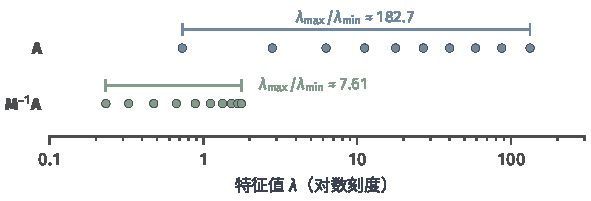
\includegraphics[width=100mm]{figures/01-basic-mathematics/03-vectors-matrices-and-multivariate-functions/matplotlib/c5-preconditioned-spectrum/figure.pdf}
  \caption{对角缩放前后的特征值分布（对数横轴）。矩阵为$\bm A=\bm S\bm T\bm S$，$\bm S=\operatorname{diag}(1,\ldots,10)$，$\bm T$为对角元$1$、次对角元$0.4$的三对角矩阵，预条件$\bm M=\operatorname{diag}(\bm A)$。蓝点为$\bm A$的$10$个特征值（数值计算），绿点为$\bm M^{-1}\bm A$的特征值$1+0.8\cos(j\pi/11)$；括线标出各自的范围与最大、最小特征值之比。}
  \label{fig:ls-preconditioned-spectrum}
\end{figure}

\paragraph{计算代价}
每轮比CG多一次$\bm M$求解，选用时要同时计入构造$\bm M$与每轮应用的成本，比较达到同一精度的总工作量。对角缩放几乎不需构造；SSOR不需额外存储因子，但每次应用相当于两次三角扫掠；不完全分解要先付出构造代价并存储因子，换来通常更接近$\bm A$的近似。

\paragraph{GMRES与MINRES的预条件}
对GMRES，左预条件在预条件后的Krylov空间中最小化$\lVert\bm M^{-1}(\bm b-\bm A\bm x)\rVert_2$，右预条件保留原残差$\lVert\bm b-\bm A\bm x\rVert_2$作为目标；两者结束时都回到第~\ref{sec:ls-stationary-stopping}节检查原残差。MINRES要求保持对称性，只能采用对称正定预条件$\bm M=\bm C\bm C^\top$的分裂变换$\bm C^{-1}\bm A\bm C^{-\top}$。预条件只改善变换后的谱，不改变原问题对数据的敏感度。

\paragraph{最小二乘目标的保持}
对不相容最小二乘问题，还要核对变换是否保持原目标。左变换给出$\lVert\bm M^{-1}(\bm b-\bm A\bm x)\rVert_2^2=(\bm b-\bm A\bm x)^\top\bm M^{-\top}\bm M^{-1}(\bm b-\bm A\bm x)$，即第~\ref{sec:ls-weighted-ls}节以$\bm M^{-\top}\bm M^{-1}$为权的加权目标，一般会改变解。可逆右变换$\bm x=\bm M^{-1}\bm y$使两个问题的残差逐点相同，原残差目标和解集都保留；但零初值在$\bm y$坐标下选出的是$\lVert\bm y\rVert_2=\lVert\bm M\bm x\rVert_2$最小的解，秩亏时它未必是原坐标下欧氏范数最小的最小二乘解。因此比较预条件时不能只比较迭代次数，还要确认所求的是不是原来那个解。

\section{收敛检验与停止准则}
\label{sec:ls-krylov-stopping}

方阵上的CG、PCG、GMRES、MINRES、BiCG与BiCGSTAB统一沿用第~\ref{sec:ls-stationary-stopping}节的规则：超参数为$\bm x_0,\mathrm{atol},\mathrm{rtol},K$，以阈值$\mathrm{atol}+\mathrm{rtol}\lVert\bm b\rVert_2$检查真实原残差$\lVert\bm b-\bm A\bm x_k\rVert_2$，达到阈值或步数上限时输出当前$\bm x$。达到上限本身不表示已经收敛。

递推残差和小问题残差只用于内部计算，决定何时值得复核，不另作算法输出。它们在精确算术下等于真实残差，浮点计算中却会逐渐偏离：CG与PCG的递推残差，GMRES的$\lvert g_{j+1}\rvert$，MINRES的$\lvert\bar g_{j+1}\rvert$，LSQR与LSMR的标量估计都是如此。所以实现中定期、并在每次候选终止前，用$\bm A,\bm b,\bm x_k$重新计算残差。

LSQR与LSMR以相容方程为目标时，可以沿用同一原残差阈值。以最小二乘为目标时，不相容问题的最优原残差不为零，原残差阈值可能永远达不到，所以单列非负超参数$\tau_n$，检查
\[
 \lVert\bm A^\top(\bm b-\bm A\bm x_k)\rVert_2\le\tau_n ,
\]
允许原残差非零。原残差的大小与正规残差是否接近零回答的是两个不同的问题：前者说明数据被拟合得多好，后者说明是否已经到达最小二乘解。$\tau_n$是绝对阈值，应与所用数据的尺度相配，不除以$\lVert\bm A^\top\bm b\rVert_2$这类可能为零的参照量。初值已满足条件时直接输出$\bm x_0=\bm0$；其余情况在每次候选终止和最终输出前都复核。达到$K$时只输出当前$\bm x$，残差和停止原因都不纳入输出。

没有达到精度而结束的情形要彼此区分。步数上限只说明不再继续计算；停滞指真实残差在若干轮内几乎不降，常见于重启GMRES；中断指BiCG、BiCGSTAB的配对量或$\omega$为零，或PCG遇到非正的分母，这时递推本身无法继续。它们都不能报告成收敛，后续是调整参数、换用预条件还是换用方法，要根据具体原因决定。

残差小的含义还要结合原问题的条件数来解释；要求最小范数解时，还须保持零初值、迭代留在行空间，并核对预条件下的选解准则。真实残差复核所需的矩阵乘法计入实际成本。误差的解释留到第~\ref{sec:ls-numerical-sensitivity}节，达到同一精度的综合比较留到第~\ref{sec:ls-method-selection}节。
